%% 
%% Skript Differentialgeometrie im Wintersemester 12/13
%% Zur Vorlesung von Dr. Grensing am KIT Karlsruhe
%% 
%% Kapitel 6
%% 

\chapter{Riemannsche Metriken}

\begin{emptythm}[Was ist Geometrie?]
Vereinfacht ausgedr"uckt suchen wir eine M"oglichkeit um Distanzen und Winkel auszudr"ucken.
Betrachte im Folgenden die Einheitssph"are, auf der wir den eine Reise von $x$ nach $y$ unternehmen m"ochten.
\begin{center}\begin{tikzpicture}
	%\draw[step=0.25,gray!15] (-4,-4) grid (4,4); \draw[step=0.5,gray!30] (-4,-4) grid (4,4); \fill (0,0) circle(0.1); %Hilfsgitter
	
	\draw (0,0) circle (3);
	\begin{scope}
		\clip (-3,0) rectangle (3,1.6);
		\draw[dashed] (0,0) ellipse (3 and 1);
	\end{scope}
	\begin{scope}
		\clip (-3,0) rectangle (3,-1.6);
		\draw (0,0) ellipse (3 and 1);
	\end{scope}
	
	\fill (0,3) circle(0.05) node[anchor=south west]{$N$};
	\fill (0,-3) circle(0.05) node[anchor=north west]{$S$};
	
	\coordinate (x) at (-0.5,2); \coordinate (y) at (0.75,-2);
	\fill (x) circle(0.05)node[above]{$x$};
	\fill (y) circle(0.05)node[below]{$y$};
	\draw (x) -- (y);
	\coordinate (a) at (1.25,0.75); \coordinate (b) at (1,0.25); \coordinate (c) at (1.5,-0.25);
	\draw (x) ..controls(x) and ($(a) + (-1.25,1.25)$).. (a) ..controls($(a) + (0.25,-0.25)$) and ($(b) + (0,0.25)$).. (b) ..controls($(b) + (0,-0.25)$) and ($(c) + (0,0.25)$).. (c) ..controls($(c) + (0,-0.75)$) and (y).. (y);
	
	\node at (2.75,2.75) {$S^2 \subset \R^3$};
	\draw[->] (1.5,-2)node[anchor=north]{$c$} to[out=90,in=310] (1.25,-1.25);
	
	\node at (-3.25,-2.5) {$c: [0,1] \to S^2$};
	\node at (-3.25,-3.25) {$c(0) = x,\quad c(1) = y$};
\end{tikzpicture}\end{center}
Wir definieren mit $\calL(c) = \int_0^1 \|\dot c\| \dop t$ die \CmMark[Metrik!Riemann-]{Riemann-Metrik}, also das Skalarprodukt mit allen $\T_pM$.
Damit folgt dass wenn $c: [0,1] \to M$ glatt ist, dass $\calL(c) = \int_0^1 \sqrt{\langle \dot c, \dot c \rangle}$ und der Abstand auf $M$ kann ausgedr"uckt werden durch $d_M(x,y) = \inf \{\calL(c) | c$ von $x$ nach $y\}$.

Das wirft Fragen auf nach der Existenz k"urzester Abst"ande, Unterschieden zwischen lokal K"urzestem und global K"urzesten und der Eindeutigkeit.
\end{emptythm}

\begin{Dfn}
  Es sei $M$ eine glatte Mannigfaltigkeit.
  Eine \CmMark[Metrik!Riemann-]{Riemannsche Metrik} $g$ auf $M$ ist gegeben durch ein Skalarprodukt auf jedem $\T_pM$, welches glatt von $p$ abh"angt, das hei"st $g \in \calT_2^0(M)$, so dass $g_p = \langle \cdot, \cdot \rangle_p : \T_pM \X \T_pM \ \to \R$ symmetrisch und positiv definit ist.
  Ist $g$ eine Riemann-Metrik auf M, so hei"st $(M,g)$ eine \CmMark[Mannigfaltigkeit!Riemannsche]{Riemannsche Mannigfaltigkeit}.
\end{Dfn}

Ist $(M,g)$ eine Riemannsche Mannigfaltigkeit, $X, Y \in \calV(M)$, $X = \sum \xi^{i} \pdifffrac{}{x^{i}}$, $Y = \sum \eta^j \pdifffrac{}{y^j}$, dann ist
\begin{align*}
  g(X, Y) & = g\left(\sum \xi^{i} \pdifffrac{}{x^{i}}, \sum \eta^j \pdifffrac{}{y^j}\right)\\
  & = \sum_{i,j}\xi^{i} \eta^j g\left(\pdifffrac{}{x^{i}}, \pdifffrac{}{y^j}\right)\\
  & = \sum_{i,j} \xi^{i} \eta^j g_{ij} \qquad (g_{ij} \text{ glatt, } g_{ij} = g_{ji})
\end{align*}

\begin{bsp}
  \begin{enumerate}[label=(\arabic*),leftmargin=*]
  \item $\R^m$ tr"agt eine nat"urliche Riemannsche Metrik: F"ur $x \in \R^m$ ist $\calI_x: \T_x\R^m \to \R^n$ ein (nat"urlicher) Isomorphismus.
    Damit definiert
    \[ g_x(\cdot,\cdot) = \langle \calI_x(\cdot,\cdot), \calI_x(\cdot,\cdot) \rangle \]
    eine Riemannsche Metrik auf $\R^m$. Bez"uglich der Karte $(\Id, \R^m)$ gilt
    \[ g_{ij} = \sum_{ij} \delta_{ij} \dop x^{i} \otimes \dop x^j = \sum_i \dop x^{i} \otimes \dop x^j \]
  \item Betrachtet man Polarkoordinaten auf $\R^2(r, \theta)$:
    \begin{align*}
      \pdifffrac[(r,\theta)]{}{r} &= (\cos \theta, \sin \theta)\\
      \pdifffrac[(r,\theta)]{}{\theta} &= r(-\sin \theta, \cos \theta)
    \end{align*}
    \begin{align*}
      g_{rr} &= g\left( \pdifffrac{}{r}, \pdifffrac{}{r} \right) = 1\\
      g_{\theta\theta} &= g\left( \pdifffrac{}{\theta}, \pdifffrac{}{\theta} \right) = r^2\\
      g_{r\theta} &= g_{\theta r} = 0
    \end{align*}
  \item Sei $M \subseteq \R^n$ $m$-dimensionale glatte Untermannigfaltigkeit. $M$ tr"agt eine nat"urliche Riemann-Metrik:
    \begin{center}\begin{tikzpicture}
        % \draw[step=0.25,gray!15] (-4,-4) grid (4,4); \draw[step=0.5,gray!30] (-4,-4) grid (4,4); \fill (0,0) circle(0.1); %Hilfsgitter
        
        \draw (0,0) circle(2);
        \begin{scope}
          \clip (-2,0) rectangle (2,2);
          \draw[dashed] (0,0) ellipse(2 and 0.75);
        \end{scope}
        \begin{scope}
          \clip (-2,0) rectangle (2,-2);
          \draw (0,0) ellipse(2 and 0.75);
        \end{scope}
        
        \path[name path=laenge] (0,2) to[out=335,in=33] (0,-2);
        \path[name path=breite] (0,2) ellipse(2 and 0.75);
        \path[name path=aequator] (0,0) ellipse(2 and 0.75);
        \path[name intersections={of=laenge and breite, by=p}];
        \path[name intersections={of=laenge and aequator, by={grenze1, grenze2}}];
        
        \coordinate (a) at (1,2.25); \coordinate (b) at (-1,0.5); \coordinate (c) at (1.75,-1.5); \coordinate (d) at ($(a) + (c) - (b)$);
        \path[draw,name path=raute] (a) -- (b) -- (c) -- (d) -- cycle;
        
        \begin{scope}
          \clip (0,2) rectangle ($(grenze2) + (0.5,0)$);
          \draw (0,2) to[out=335,in=33] (0,-2);
          \clip (0,0) circle(2);
          \draw (0,2) ellipse(2 and 0.75);
        \end{scope}
        \begin{scope}
          \clip (0,0) circle(2);
          \draw (0,2) ellipse(2 and 0.75);
        \end{scope}
        
        \node at (-2,2) {$S^2 \subset \R^3$};
        \fill (p) circle(0.05)node[anchor=south west,font=\scriptsize] at (p) {$p$};
        \draw[->] (p) -- ($(p) + 0.6*(1,-1.7)$);
        \draw[->] (p) -- ($(p) + 1.1*(1,0.15)$);
        
        \draw[->] (2.25,2.25)node[right,font=\scriptsize]{$\pdifffrac{}{\phi}$} to[out=210,in=80] (1.65,1.5);
        \draw[->] (3.25,1.25)node[right,font=\scriptsize]{$\pdifffrac{}{\theta}$} to[out=180,in=30] (1.2, 0.75);
      \end{tikzpicture}\end{center}
    F"ur jedes $p \in M$ ist $\T_pM$ kanonisch isomorph zum von partiellen Ableitungen $\partial_1F|_p, \ldots ,\partial_mF|_p$ einer lokalen Parametrisierung $F$ aufgespannten Untervektorraum $\R^m$. Mit diesem (lokalen) isomorphismus definiert
    \[ g_{ij} = \langle \partial_i F, \partial_j F \rangle \]
    eine Riemann-Metrik auf $M$.
  \end{enumerate}
\end{bsp}

\begin{bem}
  Sind $\phi$ und $\psi$ Karten einer Riemannschen Mannigfaltigkeit $(M,g)$ um $p$ und sind $g = \sum g_{ij} \dop x^{i} \otimes \dop x^j$ und $h = \sum h_{ij} \dop y^{i} \otimes \dop y^j$ die lokalen Darstellungen bez"uglich $\phi$ beziehungsweise $\psi$, so gilt
  \[ h_{kl} = g\left( \pdifffrac{}{y^k}, \pdifffrac{}{y^l} \right) = \sum_{i,j} \pdifffrac{x^{i}}{y^k} \underbrace{\pdifffrac{x^j}{y^l}}_{\mathclap{\qquad \partial_l(\phi^{i}\circ \psi^{-1})}} g_{ij} \]
\end{bem}

Eine Riemannsche Metrik induziert eine Metrik auf dem Kotangentialb"undel: Die Isomorphismen $\T_pM \to \T_p^*M$, $X \mapsto \langle X, \cdot \rangle_p$ einen Isomorphismus von $\T M$ nach $\T^*M$.
F"ur $\omega \in \T_p^*M$ sei $X(\omega) \in \T_pM$ mit $\omega = \langle X(\omega), \cdot \rangle_p$.
Man definiert nun durch
\[ \langle \omega, \tilde \omega \rangle = \langle X(\omega), X(\tilde \omega) \rangle \]
ein Skalarprodukt auf $\T_p^*M$. F"ur $\omega = \sum \omega_i \dop x^{i}$, $X(\omega) = \xi^{i} \pdifffrac{}{x^{i}}$ gilt
\[ \omega_i = \omega \left( \pdifffrac{}{x^{i}} \right) = \left\langle X(\omega), \pdifffrac{}{x^{i}} \right\rangle = \sum_j \xi^{i} g_{ij} \]
Also $\xi^{i} = \sum g^{ij} \omega_i$, wobei $(g^{ij})$ die zu $(g_{ij})$ inverse Matrix ist.
Damit gilt:
\begin{align*}
  \langle \omega, \tilde \omega \rangle &= \langle X(\omega), X(\tilde \omega) \rangle \\
  &= \sum g_{kl} \xi^k \xi^l\\
  &= \sum g_{kl} g^{ki} \omega_i g^{lj} \tilde \omega_j\\
  &= \sum \delta_l^i g^{lj} \omega_i \tilde \omega_j\\
  &= \sum g^{ij} \omega_i \tilde \omega_j\\
\end{align*}


%%%
%%% 13. Vorlesung <2012-11-27 Tue>
%%%

F"ur beliebige Tensoren $S, S' \in T_q^p(\T M)$ und $T, T' \in T_l^k(\T M)$ definiert man induktiv durch lineare Fortsetzung Skalarprodukte wie folgt:
\begin{align*}
  \left<S \otimes T, S' \otimes T'\right> = \left<S,S'\right> \otimes \left<T,T'\right>.
\end{align*}
Auf $\T M \otimes \T M$ hat die Metrik die folgende Gestalt:
\begin{align*}
  \left<X \otimes Y,\tilde X \otimes \tilde Y\right> = \sum g_{ij}g_{kl}\xi^i\tilde\xi^j\eta^k\tilde\eta^l.
\end{align*}

% Definition 6.2
\begin{Dfn}
  Es seien $(M, g)$ und $(N,h)$ Riemannsche Mannigfaltigkeiten.
Ein Diffeomorphismus $\Phi \colon M \to N$ hei"st \CmMark{Isometrie}, falls $\Phi^{*}h = g$, das hei"st f"ur alle $p \in M$ und $X,Y \in \T_pM$ gilt:
\begin{align*}
  g_p(X,Y) = \underbrace{h_{\Phi(p)}(\Phi_{*p}X,\Phi_{*p}Y)}_{\mathclap{= \Phi^{*}h(X,Y) \; \rightsquigarrow \text{Pullback Metrik}}}
\end{align*}
Ist umgekehrt $\Phi \colon M \to N$ ein Diffeomorphismus und $h$ eine Riemannsche Metrik auf $N$, so ist $\Phi^{*}h$ eine Riemannsche Metrik auf $M$.
\end{Dfn}

% Satz 6.3
\begin{Satz}\label{Satz-6-3}
  Jede glatte Mannigfaltigkeit tr"agt eine Riemannsche Metrik.
\end{Satz}

Um Metriken in den "Uberlappungsgebieten von Karten "`verkleben"' zu k"onnen, ben"otigt man das folgende Hilfsmittel.

% Hilfssatz
\begin{satz}[Zerlegung der Eins]
  Es sei $M$ eine glatte Mannigfaltigkeit und $\{U_i\}_{i \in \calI}$ eine offene "Uberdeckung von $M$.
  Dann existiert eine \CmMark{Zerlegung der Eins} auf einer abz"ahlbaren, lokal endlichen Verfeinerung von $\{U_i\}_{i \in \calI}$, das hei"st es existiert eine abz"ahlbare offene "Uberdeckung $\{V_k\}_{k\in\N}$ von $M$ und glatte Funktionen mit kompaktem Tr"ager $\alpha_k \colon M \to \R$, so dass gilt:

  \begin{enumerate}[label=(\roman*)]
  \item $\forall k \in \N \ \exists i(k) \in \calI: V_k \subseteq U_{i(k)}$ (Verfeinerung),
  \item $\forall p \in M \ \exists U \ni p: \# \{k \mid V_k \cap U \neq \emptyset \} < \infty$ (lokal endlich),
  \item $\forall k \in \N: \supp (\alpha_k) \subseteq V_k$,
  \item $\forall k \in \N \ \forall p \in M: 0 \leq \alpha(p) \leq 1$,
  \item $\forall p \in M: \sum_{k\in\N}\alpha_k(p) = 1$.
  \end{enumerate}
  (Wegen (ii) und (iii) ist die Summe in (v) endlich).
\end{satz}
An dieser Stelle geht ma"sgeblich ein, dass die Topologie von $M$ eine abz"ahlbare Basis besitzt. Beweis siehe Boothby, Kapitel V.4 \cite{boothby1986introduction}.

\begin{bew}(von Satz \ref{Satz-6-3})
Es sei $M$ eine glatte, $m$-dimensionale Mannigfaltigkeit. $\{(\phi_i,U_i)\}_{i \in \calI}$ ein Atlas von $M$ und $\{(V_k,\alpha_k)\}_{k \in \N}$ eine Zerlegung der Eins auf einer abz"ahlbaren, lokal endlichen Verfeinerung von $\{U_i\}_{i \in \calI}$. Es sei $\beta$ ein Skalarprodukt auf $\R^m$. F"ur jedes $k \in \N$ ist dann
\begin{align*}
	g_k = \left.\phi_{i(k)}\right|_{V_k}^{*}\beta
\end{align*}
eine Riemannsche Metrik auf $V_k$. Damit ist $g = \sum g_k\alpha_k$ eine Riemannsche Metrik auf $M$.
Die Summe ist punktweise endlich und $g$ ist als Komposition glatter Abbildungen selbst glatt.
Symmetrie und Bilinearit"at folgen sofort.
F"ur jedes $p \in M$ gilt $\sum_{k \in \N}\alpha_k(p) = 1$, das hei"st es existiert ein $l \in \N$ mit $\alpha_l(p) > 0$ und f"ur $X \in \T_pM$ mit $X \neq 0$ folgt:
\begin{align*}
	g_p(X,X) & = \sum \underbrace{g_k(p)(X,X)}_{> 0}\alpha_k(p)\\
	& \geq g_l(p)(X,X)\alpha_l(p) > 0.
\end{align*}
Damit ist $g$ positiv definit.
\end{bew}

F"ur eine glatte Kurve $\gamma \colon [a,b] \to M$ hei"st
\begin{align*}
  \mathcal L(\gamma) = \int_{a}^b\|\dot \gamma\| = \int_a^b \sqrt{g_{\gamma(t)}(\dot\gamma(t),\dot\gamma(t))}\dop t
\end{align*}
die \CmMark[L\"ange!Kurven-]{(Kurven-)L"ange} von $\gamma$. Ist $\tau \colon [\alpha,\beta] \to [a,b]$ glatt und monoton, so gilt\marginnote{\textcolor{gray}{\scriptsize{$\tau'$ ist die Ableitung von $\tau$, der Strich wurde aus "asthetischen Gr"unden statt dem Punkt gew"ahlt}}}
\begin{align*}
  \mathcal L(\gamma \circ \tau) & = \int_{\alpha}^{\beta}\|\dot\gamma(\tau(s))\||\tau'(s)|\dop s\\
  & = \int_a^b\|\dot\gamma\| = \mathcal L(\gamma).
\end{align*}
Damit ist die Kurvenl"ange invariant unter Reparametrisierungen. Ist $\gamma$ \CmMark[regul\"ar!Kurve]{regul\"ar}, das hei"st $\dot\gamma(t) \neq 0$ f"ur alle $t \in [a,b]$, so ist ihre sogenannte \CmMark{Bogenl"ange}
\begin{align*}
  \sigma \colon [a,b] \to [0,\mathcal L(\gamma)], t \mapsto \mathcal L(\gamma|_{[a,t]}) = \int_a^t\|\dot\gamma\|.
\end{align*}
streng monoton steigend, also $\sigma'(s) = \|\dot\gamma(s)\| > 0$.
F"ur $\tilde\gamma = \gamma \circ \sigma^{-1}\colon [0,\mathcal L(\gamma)] \to M$ gilt $\|\dot{\tilde\gamma}\| \equiv 1$.
Die Kurve $\tilde \gamma$ hei"st \CmMark{Bogenl"angenparametrisierung} von $\gamma$.
Gilt f"ur $\gamma \colon [a,b] \to M$ dass $\|\dot\gamma\| \equiv \lambda$, so hei"st $\gamma$ \CmMark[Parametrisierung!proportional zur Bogenl"ange]{proportional zur Bogenl"ange} parametrisiert.

\marginnote{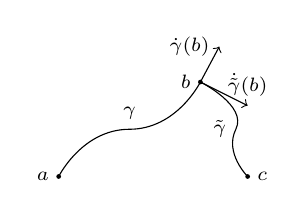
\begin{tikzpicture}[font=\scriptsize,scale=0.6]
	%\draw[step=0.25,gray!15] (-4,-4) grid (4,4); \draw[step=0.5,gray!30] (-4,-4) grid (4,4); \fill (0,0) circle(0.1); %Hilfsgitter
	\fill (0,0) circle(0.05)node[left]{$b$} (-3,-2) circle(0.05)node[left]{$a$} (1,-2) circle(0.05)node[right]{$c$};	
	\draw (-3,-2) ..controls(-3,-2) and (-2.5,-1).. (-1.5,-1)node[above]{$\gamma$} ..controls(-0.5,-1) and (0,0).. (0,0);
	\draw (0,0) ..controls(0,0) and (1,-0.5).. (0.75,-1)node[left]{$\tilde\gamma$} ..controls(0.5,-1.5) and (1,-2).. (1,-2);
	\draw[->] (0,0) -- (0.4,0.75)node[left]{$\dot\gamma(b)$};
	\draw[->] (0,0) -- (1,-0.5)node[above]{$\dot{\tilde\gamma}(b)$};
\end{tikzpicture}}
Sind $\gamma \colon [a,b] \to M, \tilde \gamma \colon [b,c] \to M$ glatte Kurven mit $\gamma(b) = \tilde \gamma(b)$, so sei
\begin{align*}
  \mathcal L(\gamma \cup \tilde\gamma) = \mathcal L(\gamma) + \mathcal L(\tilde \gamma).
\end{align*}
Eine Kurve $\gamma \colon [a,b] \to M$ hei"st \CmMark{st"uckweise glatt}, wenn $t_0, \ldots, t_k$ mit $a = t_0 < t_1 < \cdots < t_k = b$ existieren, so dass $\gamma|_{[t_{i-1},t_i]}$ f"ur alle $i \leq k$ glatt ist.

% Definition 6.4
\begin{Dfn}
  F"ur Punkte $p, q \in M$ ist der \CmMark{Abstand} definiert durch:
  \begin{align*}
    \dop(p,q) = \inf\{ \mathcal L(\gamma) \mid \gamma \colon [0,1] \to M \text{ st"uckweise glatt mit } \gamma(0) = p, \gamma(1) = q\}.
  \end{align*}
\end{Dfn}

% Satz 6.5
\begin{Satz}
  Es sei $(M,g)$ eine zusammenh"angende Riemannsche Mannigfaltigkeit.
  Die Abstandsfunktionen bilden eine Metrik auf $M$, welche die urspr"ungliche Topologie induziert.
\end{Satz}

Der Beweis sei zur "Ubung "uberlassen.

% Satz 6.6
\begin{Satz}
  Es seien $(M,g)$ und $(N,h)$ zusammenh"angende Riemannsche Mannigfaltigkeiten und $\Phi \colon M \to N$ ein Diffeomorphismus.
  Dann ist $\Phi$ genau dann eine Isometrie, wenn $\mathcal L(\Phi \circ \gamma) = \mathcal L(\gamma)$ f"ur alle glatten $\gamma \colon [0,1] \to M$ gilt. 
\end{Satz}

\begin{bew}
  Dass eine Isometrie die Kurvenl"angen erh"alt gilt offensichtlich. Erh"alt $\Phi$ die Kurvenl"angen, so erh"alt $\Phi$ auch die Norm von Tangentialvektoren, den andernfalls g"abe es $X_p \in \T_pM$ mit (ohne Einschr"ankung)
  \begin{align*}
    h_{\Phi(p)}(\Phi_{*p}X,\Phi_{*p}X) > g_p(X,X)
  \end{align*}
  und eine Kurve $\gamma\colon [0,1] \to M$ mit $\gamma(0) = X$ und es g"alte (f"ur hinreichend kleines $\epsilon$):
  \begin{align*}
    \mathcal L(\gamma|_{[0,\epsilon]}) & = \int_0^{\epsilon}\sqrt{g_{\gamma(t)}\left(\dot\gamma(t),\dot\gamma(t)\right)}\dop t\\
    & < \int_0^{\epsilon}\sqrt{h_{\Phi(\gamma(t))} \left(\Phi_{*\gamma(t)}\dot\gamma(t), \Phi_{*\gamma(t)}\dot\gamma(t)\right)}\dop t\\
    & = \int_0^{\epsilon}\sqrt{h_{\Phi(\gamma(t))} \left(\dot{(\Phi \circ \gamma)}(t), \dot{(\Phi \circ \gamma)}(t) \right)}\dop t\\
    & = \mathcal L \left((\Phi \circ \gamma)|_{[0,\epsilon]}\right).
  \end{align*}
  Mit der Polarisationsformel $\left<x,y\right> = - \frac{1}2 (\|x-y\|^{2} - \|x\|^2-\|y\|^2)$ folgt dann, dass $\Phi$ auch die Skalarprodukte erh"alt.
\end{bew}

% Definition 6.7
\begin{Dfn}
  Eine Kurve $\gamma \colon [a,b] \to M$ hei"st \CmMark[Geod\"atische!minimale]{minimale Geod"atische} von $\gamma(a)$ nach $\gamma(b)$, falls ein $\lambda \geq 0$ existiert, so dass f"ur alle $a \leq s < t \leq b$ gilt:
  \begin{align*}
    \mathcal L(\gamma|_{[s,t]}) = \lambda(t-s) = \dop(\gamma(s),\gamma(t)).
  \end{align*}

  Eine Kurve $\gamma$ hei"st \CmMark{Geod\"atische}, falls sie lokal minimierende Geod"atische ist, das hei"st f"ur alle $t \in [a,b]$ existiert ein $\epsilon > 0$, so dass $\gamma|_{[t-\epsilon,t+\epsilon]}$ minimierende Geod"atische ist.
\end{Dfn}

Eine bessere Vorstellung erh"alt man durch Betrachtung von Geod"atischen als Isometrien von Intervallen in den euklidischen Raum, denn $\dop(\gamma(s),\gamma(t)) = t-s = \dop_{\R}(t,s)$.

\begin{center}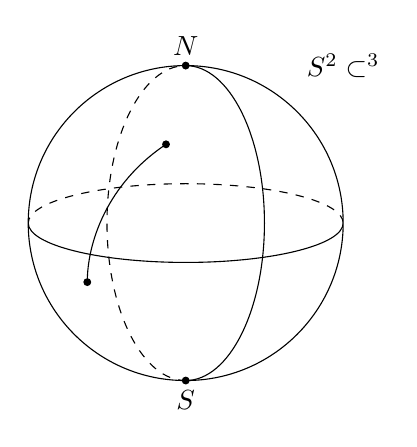
\begin{tikzpicture}
    % \draw[step=0.25,gray!15] (-4,-4) grid (4,4); \draw[step=0.5,gray!30] (-4,-4) grid (4,4); \fill (0,0) circle(0.1); %Hilfsgitter
    \draw (0,0) circle (2);
    \fill (0,2) circle(0.05)node[above]{$N$} (0,-2) circle(0.05)node[below]{$S$};
    \def\vert{0.5}
    \begin{scope}
      \clip (-2,0) rectangle (2,-2);
      \draw (0,0) ellipse(2 and \vert);
    \end{scope}\begin{scope}
      \clip (-2,0) rectangle (2,2);
      \draw[dashed] (0,0) ellipse(2 and \vert);
    \end{scope}\begin{scope}
      \clip (0,-2) rectangle (2,2);
      \draw (0,0) ellipse(1 and 2);
    \end{scope}\begin{scope}
      \clip (0,-2) rectangle (-2,2);
      \draw[dashed] (0,0) ellipse(1 and 2);
    \end{scope}
    
    \fill (-1.25,-0.75) circle (0.05) (-0.25,1) circle (0.05);
    \draw (-1.25,-0.75) ..controls(-1.25,-0.25) and (-1,0.5).. (-0.25,1);
    
    \node at (2,2) {$S^2 \subset \R^3$};
  \end{tikzpicture}\\
  Geod"atische = Gro"skreissegmente\end{center}


%%% 
%%% 14. Vorlesung <2012-11-30 Fri>
%%% 

\begin{bem}
  \begin{enumerate}[label=(\arabic*),leftmargin=*]
  \item Die Geod"atischen von $\R^n$ mit Standardmetrik sind genau die Geradensegmente.
  \item Ist $\gamma$ eine minimale Geod"atische, so gilt $\|\dot\gamma\| = \lambda$, falls $\lambda > 0$, existiert eine Bogenl"angenparametrisierung $\tilde\gamma$ von $\gamma$ auf $[0,l]$ mit $l = \mathcal L(\gamma) = \mathcal L(\tilde\gamma)$ und $\dop(\tilde\gamma(0),\tilde\gamma(t)) = t$.
    Damit ist $\tilde\gamma$ eine isometrische Einbettung von $[0,l]$ in $M$.
  \end{enumerate}
\end{bem}

% Definition 6.8
\begin{Dfn}
  Es sei $\gamma \colon [a,b] \to M$ eine (st"uckweise) glatte Kurve auf $M$.
  Das Integral
  \begin{align*}
    E(\gamma) = \frac{1}2 \int_a^b\|\dot\gamma\|^2
  \end{align*}
  hei"st \CmMark{Energie} von $\gamma$.
\end{Dfn}

% Lemma 6.9
\begin{Lemma}\label{lemma-6-9}
  F"ur eine (st"uckweise) glatte Kurve $\gamma \colon [0,1] \to M$.
  Dann gilt:
  \begin{align*}
    \frac{1}2 \mathcal L(\gamma)^2 \leq E(\gamma),
  \end{align*}
  wobei Gleichheit genau dann gilt, wenn $\gamma$ proportional zur Bogenl"ange parametrisiert ist.
\end{Lemma}

\begin{bew}
  Es gilt die Cauchy-Schwarzsche Ungleichung f"ur das Skalarprodukt $(f,g) \mapsto \int_0^1 fg$ mit $f,g \in \C^{\infty}([0,1], \R)$.

  Nun sei $f \equiv 1$ und $g = \|\dot\gamma\|$, so folgt:
  \begin{align*}
    \mathcal L(\gamma) = \int_0^1 \|\dot\gamma\| \leq \left|\left(\int_0^1 f^2\right)^{\frac{1}2} \left(\int_0^1g^2\right)^{\frac{1}2}\right| = \sqrt{2 E(\gamma)}
  \end{align*}
  Gleichheit gilt genau dann, wenn $1$ und $\|\dot\gamma\|$ $\R$-linear abh"angig sind, das hei"st wenn $\|\dot\gamma\| \equiv \lambda$ gilt.
\end{bew}

% Satz 6.10
\begin{Satz}
  Eine (st"uckweise) glatte Kurve ist genau dann minimale Geod"atische, wenn ihre Energie minimal ist.
\end{Satz}

\begin{bew}\begin{description}[font=\normalfont]
  \item[\quot{$\Rightarrow$}:]
    Es sei $\gamma$ minimale Geod"atische, das hei"st $\mathcal L(\gamma|_{[0,t]}) = \lambda t = \dop (\gamma(0),\gamma(t))$.
    Also gilt $E(\gamma) = \frac{1}2 \mathcal L(\gamma)^2 \leq \frac{1}2 \mathcal L(c)^2 \leq E(c)$, wobei $c$ eine Kurve zwischen den Endpunkten von $\gamma$ ist und die letzte Ungleichung aus Lemma \ref{lemma-6-9} folgt.
  \item[\quot{$\Leftarrow$}:]
    Sei $\gamma$ energieminimierend.
    \begin{align*}
      \frac{1}2 \dop (\gamma(0), \gamma(1))^2 \leq \frac{1}2 \calL(\gamma)^2 \leq E(\gamma) \leq E(\underbrace{c_n}_{\mathclap{\text{regul"are Kurven}}}) = \frac{1}2 \mathcal L(c_n)^2 \xrightarrow{n\to\infty} \frac{1}2 \dop(\gamma(0),\gamma(1))^2
    \end{align*}
    \begin{center}\begin{tikzpicture}
        % \draw[step=0.25,gray!15] (-6,-4) grid (6,4); \draw[step=0.5,gray!30] (-6,-4) grid (6,4); \fill (0,0) circle(0.1); %Hilfsgitter,
        
        \coordinate (1) at (-0.5,0.5); \coordinate (2) at (0,1.55); \coordinate (3) at (0.5,0.5);
        \coordinate (ctrl1) at (-1,-1.5); \coordinate (ctrl3) at (1,-1.5);
        \draw (-6,-1.5) ..controls(-6,-1.5) and ($(1) + (ctrl1)$).. (1) ..controls($(1) - 1/3*(ctrl1)$) and (2).. (2) ..controls(2) and ($(3) - 1/3*(ctrl3)$).. (3) ..controls($(3) + (ctrl3)$) and (6,-1.5).. (6,-1.5);
        
        \coordinate (4) at (0,0.75);
		\draw[very thick] (1) ..controls($(1) - 1/3*(ctrl1)$) and (2).. (2) ..controls(2) and ($(3) - 1/3*(ctrl3)$).. (3) ..controls($(3) - 1/15*(ctrl3)$) and ($(4) + (0.25,0)$).. (4) ..controls($(4)-(0.25,0)$) and ($(1) - 1/15*(ctrl1)$).. (1) -- cycle;
		
		\draw[dashed] (0,1.25) circle(1.25); \node[font=\scriptsize] at (0,2) {$c(t_i)$}; \node at (3,2) {$U$ Kartenumgebung};
		\node[font=\scriptsize] at (0,-1.25) {Die L"ange des fetten Dreiecks wird beliebig klein};
	\end{tikzpicture}\end{center}

	Damit gilt: $\mathcal L(\gamma) = \dop(\gamma(0),\gamma(1))$ und wegen Cauchy-Schwarz ist $\gamma$ proportional zur Bogenl"ange parametrisiert.
	Wendet man dieses Argument auf beliebige Teilst"ucke an, erh"alt man:
	\begin{align*}
		\mathcal L(\gamma|_{[s,t]}) = \dop(\gamma(s),\gamma(t)) = \lambda(s-t).
	\end{align*}
\end{description}\end{bew}

%%% Local Variables: 
%%% mode: latex
%%% TeX-master: "../skript-diffgeom"
%%% End: 
